\documentclass[11pt,a4paper]{mwart}
\usepackage[english,polish]{babel}
\usepackage[T1]{fontenc}
\usepackage[UTF8]{inputenc}
\usepackage{polski}
\usepackage{amsmath}
\usepackage{euler}
\usepackage{plain}
\usepackage{graphicx}
\usepackage{tikz}
\title{Aplikacja dla dyspozytora}
\author{Andrzej Samson, Jędrzej Wiśniewski}
\date{\today}

\begin {document}
\maketitle
\section{Zadanie} 
Celem zadania jest stworzenie aplikacji dla dyspozytora, w której będzie można przydzielać zlecenia do samochodów w firmie. W aplikacji możliwe będzie zobaczenie miejsca, w którym znajduje się kierowca, do jakiego punktu zmierza, ile mu to zajmie czasu oraz masa jego ładunku. Dyspozytor z poziomu aplikacji będzie miał możliwość przerwania podróży samochodu i wysłanie go natychmiastowo do bazy. Samochód w punkcie do którego dotarł może zostawić część swojego towaru. Aplikacja będzie uwzględniać czas jaki należy pokonać między kolejnymi punktami, cykl pracy kierowcy oraz przerwy jakie musi zrobić. Odległości między punktami będą podawane w czasie, jaki samochód potrzebuje, aby pokonać dany odcinek drogi. Ładowność samochodu podawana będzie w kilogramach. Odległości między punktami będą stałe.
\subsection{Problem komiwojażera}
Problem polega na optymalizacji trasy, czyli znalezieniu trasy do podróży w taki sposób, aby każdy punkt tej trasy odwiedzić tylko raz i to jak najbardziej optymalnie, czyli np. żeby koszt był jak najmniejszy lub podróż trwała jak najkrócej. Problem ten zalicza się do NP-trudnych, czyli takich, gdzie ciężko jest znaleźć algorytm rozwiązujący ten problem, który jest najbardziej optymalny i najlepszy. Dlatego często rozwiązuje się takie problemy, znajdując rozwiązanie przybliżone do tego najbardziej optymalnego.
\section{Specyfikacja}
Nasza firma dostawcza oraz główna baza znajdują się w Łodzi. Stąd będą rozpoczynać trasę wszystkie samochody i załatwiać przypisane im zlecenia. Jest to też miejsce do którego muszą wrócić po wyznaczonym okresie lub gdy dyspozytor wyda im polecenie powrotu. 
\subsection{Samochody i towar}
Firma ma do dyspozycji \textit{N} samochodów dostawczych, każdy o ładowności 1000 kg. Aby samochód wyruszył z bazy nie musi być w pełni załadowany, gdyż celem jest jak najbardziej optymalna realizacja zleceń. Dopuszczalny jest również tzw. pusty przebieg, czyli podróż bez towaru do jakiegoś punktu (miejscowości), aby wypełnić zlecenie lub w przypadku powrotu do bazy, gdy dyspozytor wyda polecenie powrotu bezpośredniego. Czas pracy samochodu to 10 godzin. Po tym czasie samochód musi się zatrzymać na 14 godzinną przerwę, zanim znowu będzie mógł ruszyć w trasę. Samochód nie może wziąć takiej liczby towarów, która przekroczyłaby jego ładowność. Przeładunek towaru jest natychmiastowy (nie zabiera dodatkowego czasu).
\subsection{Miejscowości i trasa}
Na \textit{rysunku 1} przedstawiona została mapa Polski na której zaznaczone są miejscowości do których podróżują samochody firmowe, punkty łączące dane odcinki oraz trasy między nimi jakie mają do pokonania. Wszystkie zaznaczone odcinki posiadają przypisany numer oraz czas podróży między dwoma punktami. W celu znalezienia najbardziej optymalnej trasy, aplikacja będzie znajdować wszystkie możliwe drogi, aby dotrzeć do punktu końcowego, sumować czas jaki należy pokonać między danymi odcinkami, porównywać je między sobą, a następnie wyświetlać najszybsze trasy podróży. Dla firmy najważniejszym celem jest jak najszybsze wypełnienie zlecenia.
\begin{figure}[th]
\centering
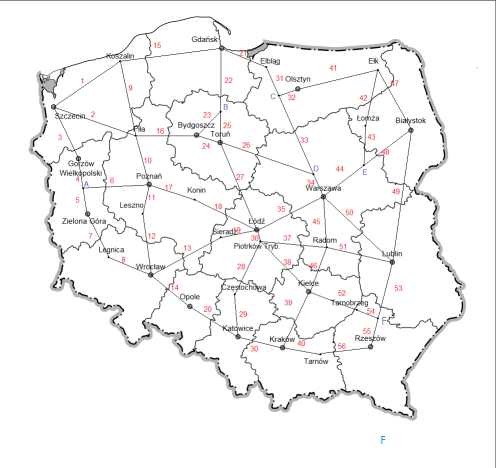
\includegraphics[width=\textwidth]{mapa.png}
\caption{Mapa miejscowości i tras razem z numeracja}
\end{figure}
\subsection{Dyspozytor i interfejs}
Dyspozytor jest \textbf{użytkownikiem} aplikacji. Może on poprzez aplikacje tworzyć nowe zlecenia - przydzielać masę towaru jaka ma być z danej miejscowości pobrana oraz do której miejscowości ją zawieźć. Dyspozytor przydziela samochody do zlecenia. Może też zawrócić samochód do bazy. Jeżeli taki samochód ma towar to dyspozytor decyduje czy zostawia go w najbliższej miejscowości, czy bierze ze sobą. Jeżeli po komendzie powrotu samochód jest pusty to wykonuje on pusty przebieg. 
Poprzez interfejs dyspozytor ma dostęp do:
\begin{flushleft}
\begin{enumerate}
\item[• Samochody] - wgląd do opisu samochodu, czyli na jakiej trasie jest samochód, masę towaru jaki ze sobą wiezie, jakie wykonuje zlecenie i ile czasu pozostało mu do zakończenia zlecenia i powrotu do bazy. W tym miejscu będzie również możliwość odesłania samochodu bezpośrednio z powrotem do bazy.
\item[• Zlecenia] - wgląd do opisu zleceń, czyli liczba przewożonego towaru, jaki samochód wykonuje to zlecenie oraz ile czasu zajmie jeszcze jego wykonanie. W tym miejscu będzie również możliwość dodawania nowych zleceń.
\item[• Mapa] - wgląd do mapy, czyli podane miejscowości oraz trasy do pokonania które są oparte na większych miejscowościach wojewódzkich i trasach krajowych.
\item[• Opcje] - opcje aplikacji
\item[• Help] - pomoc do aplikacji (FAQ)
\end{enumerate}
\end{flushleft}
\section{Algorytm}
W naszej aplikacji będziemy używać algorytmu Dijkstry. Służy on do wyznaczania najmniejszej odległości od ustalonego punktu do wszystkich pozostałych, ustalonych w grafie. W algorytmie tym pamiętany jest zbiór Q wierzchołków, dla których nie obliczono jeszcze najkrótszych ścieżek, oraz wektor D[i] odległości od wierzchołka początkowego do \textit{i}. Algorytm przebiega następująco:
\begin{flushleft}
\begin{enumerate}
\item[a]. Dopóki zbiór Q nie jest pusty wykonuj:
\item[b]. Pobierz ze zbioru Q wierzchołek \textit{v} o najmniejszej wartości D[v] i usuń go ze zbioru.
\item[c]. Dla każdego następnika \textit{i} wierzchołka v dokonaj relaksacji ścieżki, tzn. sprawdź, czy D[i]>D[v]+A[v,i], tzn czy aktualne oszacowanie odległości do wierzchołka \textit{i} jest większe od oszacowania odległości do wierzchołka \textit{v} plus waga krawędzi (v,i).
Jeżeli tak jest, to zaktualizuj oszacowanie D[i] przypisując mu prawą stronę nierówności (czyli mniejszą wartość).\\
\end{enumerate}
\end{flushleft}
Z algorytmu Dijkstry można skorzystać przy obliczaniu najkrótszej drogi do danej miejscowości. Wystarczy przyjąć, że każdy z punktów skrzyżowań dróg to jeden z wierzchołków grafu, a odległości między punktami to wagi krawędzi.
\subsection{Pseudokod}
\begin{flushleft}
Dijkstra(G,w,s):\\
dla każdego wierzchołka v w V[G] wykonaj\\
d[v] := nieskończoność\\
poprzednik[v] := niezdefiniowane\\
d[s] := 0\\
Q := V\\
dopóki Q niepuste wykonaj\\
u := Zdejmij-Min(Q)\\
dla każdego wierzchołka v – sąsiada u wykonaj\\
jeżeli d[v] > d[u] + w(u, v) to\\
d[v] := d[u] + w(u, v)\\
poprzednik[v] := u"\\
Wyświetl("Droga wynosi: " + d[v])\\
\end{flushleft}
\subsection{Graf i przykład}
\begin{flushleft}
Obliczenia przebiegają następująco: (Dla S=a)\\
(gwiazdka oznacza symbol nieskończoności, najlżejszy wierzchołek jest podkreślony, wierzchołki, dla których wyznaczono już najkrótsze ścieżki są pogrubione). Jako \textit{s} oznaczono wierzchołek początkowy.
\end{flushleft}
\begin{figure}[bh]
\centering
\includegraphics[width=0.3\textwidth]{dijkstra&tabela.png}
\caption{Graf przedstawiający wierzchołki i wektory oraz wyniki zamieszczone w tabeli}
\end{figure}
\section{Baza danych}
Aplikacja będzie korzystać z baz danych SQL-owych. Skrypt do naszej bazy jest zapisany za pomocą SQlite. \textit{Rysunek 3} przedstawia model relacyjny bazy danych, z której korzystać będzie aplikacja.
Z bazy danych aplikacja będzie otrzymywać informacje o:
\begin{enumerate}
\item[• Samochody]
\item[• Wierzchołki mapy]
\item[• Zlecenia]
\item[• Wykonanie zleceń]
\item[• Zakończenie zlecenia oraz zdarzenia nadzwyczajne]
\end{enumerate}
\begin{figure}[th]
\centering
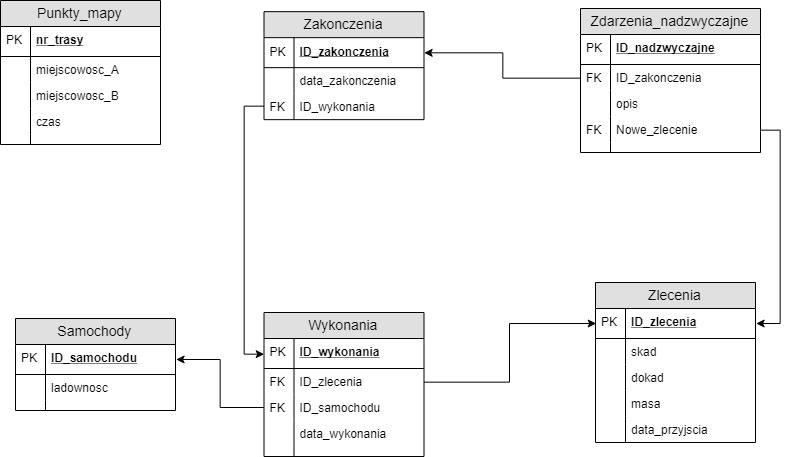
\includegraphics[width=\textwidth]{baza_model_relacyjny.jpg}
\caption{Model relacyjny bazy danych}
\end{figure}
\end {document}